\section{User Profile}

\subsection{Proximity Approach}

\begin{frame}[red] %hmm.. thought i could change colour here :S
\frametitle{Motivation}
\textsc{FriendLocator}
\begin{itemize}
	\item the Proximity Detection Guaranties is to weak $(2d\sqrt{2})$
	\item is too inflexible - privacy \& precision not independent.
\end{itemize}

\vspace{2em}

Want solution independent of how the space it partitioned
\end{frame}

\subsection{Improvements}

\begin{frame}[red] %hmm.. thought i could change colour here :S
\frametitle{Improvements}

New features and improvements in \textsc{VicinityLocator}
\begin{columns}
\begin{column}{0.5\textwidth}
\begin{itemize}
	\item Granules (and rasterasation) 
	\item Better guaranties
	\item Ajustable vicinity
\end{itemize}
\vspace{5cm}
\end{column}
\begin{column}{0.5\textwidth}
\pgfputat{\pgfxy(0,0)}{\pgfbox[left,top]{\includegraphics[width=\textwidth]{images/granVic}}}
\end{column}
\end{columns}
\end{frame}



% \subsection{VicinityLocator Examples}
% \begin{frame}[red] %hmm.. thought i could change colour here :S
% \frametitle{Demo of \textsc{VicinityLocator}}%r=500
% 	\only<1>{ 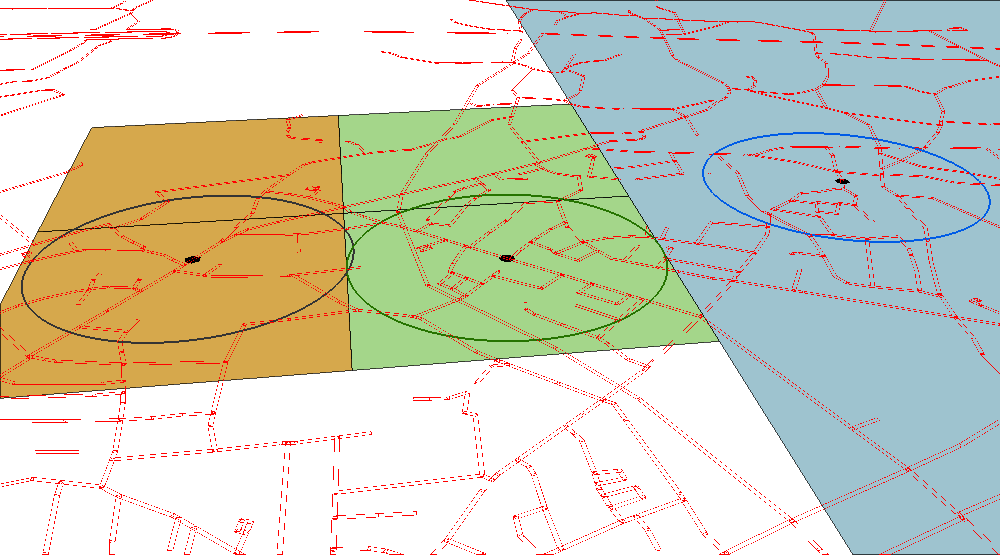
\includegraphics[page=1,scale=0.70]{images/demoVL/dump1.pdf}}
% 	\only<2>{ \includegraphics[page=1,scale=0.70]{images/demoVL/dump2.pdf}}
% 	\only<3>{ \includegraphics[page=1,scale=0.70]{images/demoVL/dump3.pdf}}
% 	\only<4>{ \includegraphics[page=1,scale=0.70]{images/demoVL/dump4.pdf}}
% 	\only<5>{ \includegraphics[page=1,scale=0.70]{images/demoVL/dump5.pdf}}
%   \only<6>{ \includegraphics[page=1,scale=0.70]{images/demoVL/dump6.pdf}}	
%   \only<7>{ \includegraphics[page=1,scale=0.70]{images/demoVL/dump7.pdf}}	
%   \only<8>{ 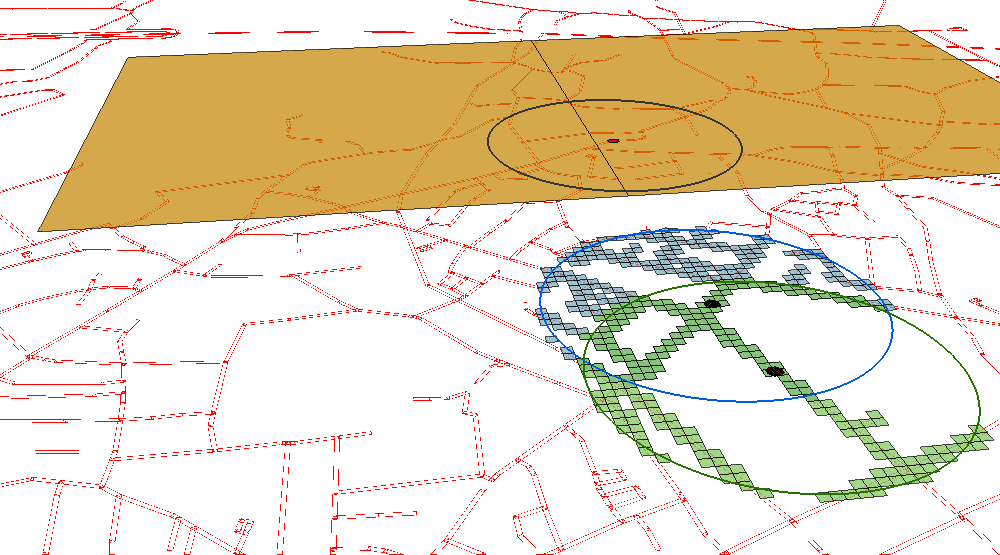
\includegraphics[page=1,scale=0.70]{images/demoVL/dump8.pdf}}	  
% \end{frame}
% 
% 
% \begin{frame}[red] %hmm.. thought i could change colour here :S
% \frametitle{\textsc{VicinityLocator} with Roadnetwork Filter}
% 
% \end{frame}
% 
% 
% \begin{frame}[red] %hmm.. thought i could change colour here :S
% \frametitle{Demo of \textsc{VicinityLocator} with Roadnetwork Filter}% R=800, Lmax = 8}
% 	\only<1>{ \includegraphics[page=1,scale=0.70]{images/demoVLRN/dump2.pdf}}
% 	\only<2>{ \includegraphics[page=1,scale=0.70]{images/demoVLRN/dump3.pdf}}
% 	\only<3>{ \includegraphics[page=1,scale=0.70]{images/demoVLRN/dump4.pdf}}
% 	\only<4>{ \includegraphics[page=1,scale=0.70]{images/demoVLRN/dump5.pdf}}
%   \only<5>{ \includegraphics[page=1,scale=0.70]{images/demoVLRN/dump6.pdf}}	
%   \only<6>{ \includegraphics[page=1,scale=0.70]{images/demoVLRN/dump7.pdf}}		  
% \end{frame}
% 
% \begin{frame}[red] %hmm.. thought i could change colour here :S
% \frametitle{\textsc{VicinityLocator} with Incremental Update}
% 
% \begin{columns}
% \begin{column}{0.5\textwidth}
% \begin{itemize}
% \item Incremental Update
% \end{itemize}
% \vspace{5cm}
% \end{column}
% \begin{column}{0.5\textwidth}
% \pgfputat{\pgfxy(0,0)}{\pgfbox[left,top]{\includegraphics[width=1.1\textwidth]{images/incUpdDemo.pdf}}}
% \end{column}
% \end{columns}
% \end{frame}
% 
% 
% \begin{frame}[red] %hmm.. thought i could change colour here :S
% \frametitle{\textsc{VicinityLocator} with Incremental Update}
% 
% \begin{columns}
% \begin{column}{0.5\textwidth}
% \begin{itemize}
% \item Incremental Update \& Roadnetwork Filter
% \end{itemize}
% \vspace{5cm}
% \end{column}
% \begin{column}{0.5\textwidth}
% \pgfputat{\pgfxy(0,0)}{\pgfbox[left,top]{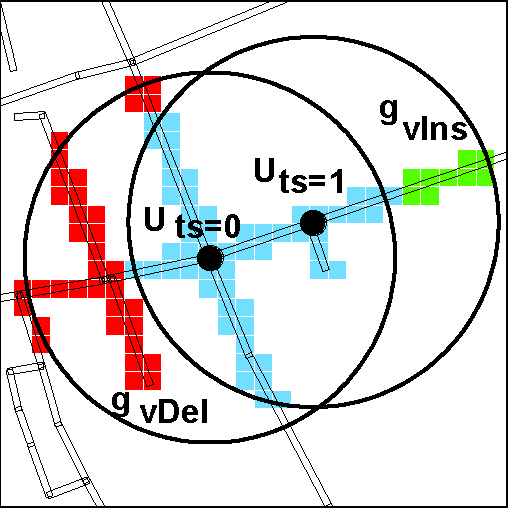
\includegraphics[width=1.1\textwidth]{images/incUpdDemo2.pdf}}}
% \end{column}
% \end{columns}
% \end{frame}